\section{Systematic Uncertainties in the Flux Prediction and Cross Section Model}
\label{sec:fluxxsecsyst}

There are three major sources of systematic uncertainty in our measurement:

\begin{itemize}
\item Flux prediction uncertainty
\item Cross section model simulation uncertainty
\item Detector level uncertainties caused by imperfect detector simulation
\end{itemize}

In this section, we describe the treatment of the first two sources of uncertainty, the flux prediction and the cross section model. Section \ref{sec:FluxDetermination} outlined the methodology behind extracting the uncertainty on the netrino flux at ND280. In Section \ref{sec:fluxsyst}, we complete the treatment of the flux uncertainty by propagating it through to our cross section measurement. Similarly, Section \ref{sec:evsim} discussed the parametrization and evaluation of the cross section model uncertainties and in Section \ref{sec:xsecsyst} we propagate these through to our measurement.

\subsection{Flux Prediction Systematic Uncertainty}
\label{sec:fluxsyst}

The flux systematic uncertainty is a large source of error in the cross section measurement. The majority of the uncertainty is due to the hadronic interaction model used with some small contribution from uncertainties in the proton beam alignment/angle and the horn current and field. As described in Section \ref{sec:FluxDetermination}, the flux uncertainty is parametrized by normalization factors in bins of neutrino or anti-neutrino energy. The $\nu_\mu$ flux is divided into 11 bins, the anti-$\nu_\mu$ into 5 bins, the $\nu_e$ into 7 bins and the anti-$\nu_e$ into 2 bins. The bin limits used are as follows (in GeV):

\begin{itemize}
\item $\nu_\mu$: 0, 0.4, 0.5, 0.6, 0.7, 1.0, 1.5, 2.5, 3.5, 5.0, 7.0, 30.0
\item anti-$\nu_\mu$: 0, 0.7, 1.0, 1.5, 2.5, 30.0
\item $\nu_e$: 0, 0.5, 0.7, 0.8, 1.5, 2.5, 4.0, 30.0
\item anti-$\nu_e$: 0, 2.5, 30.0
\end{itemize}

To propagate the flux error to our measurement, we use a 25 by 25 covariance matrix that encodes the current constraints on and correlations between the flux parameters. Figure \ref{fig:fluxcov} from Section \ref{sec:FluxDetermination} shows the flux covariance matrix used with bins for each of the neutrino types for ND280 and Super-K. The 25 bins at the bottom left of the flux covariance matrix shown are the ND280 flux bins that are used, the remainder are Super-K flux bins. We use a Cholesky decomposition technique \cite{chol} on the correlation matrix and multiply the resulting lower triangular matrix with a vector of 25 uncorrelated, gaussian, random values. The gaussians are centered at 1 and have a variance equal to the known variance of the corresponding flux bin. Each random vector multiplied by the decomposed correlation matrix yields a properly correlated ``throw'' of flux bin weights. When each flux bin weight is multiplied by the integrated flux in the given bin, each throw can be thought of as a new flux prediction. So for every new flux prediction, we have to recalculate the cross section value we aim to measure, and after many repeated throws, we produce a distribution of possible cross section measurements. The variance of this distribution tells us the uncertainty in our cross section measurement due to the uncertainty in the flux prediction at ND280. The Cholesky decomposition technique is a common mathematical tool and we use an implementation of the algorithm created by a T2K collaborator. The remainder of the flux uncertainty propagation is our work.

To recalculate the cross section for each flux throw, we re-evaluate six pieces of the cross section formula in \ref{eqn:xsec6}. We re-weight the MC and recalculate the background terms, efficiency terms and integrated flux terms. The same covariance matrix is used for all 4 beam runs. To reweight the integrated flux term, we first integrate the neutrino flux within the energy range of each $\nu_\mu$ flux bin. This integrated value is multiplied by the corresponding element, $w(i)$, of the thrown 25-element vector. This yields the new neutrino flux in that particular bin. We integrate over all 11 $\nu_\mu$ bins to calculate the new total flux as follows.

\begin{equation}
\Phi_{tot} = \sum_{i}^{11} \Phi^{new}(i) = \sum_{i}^{11} \left( w(i) \int^{bin\:hi\:edge}_{bin\:low\:edge} \Phi^{old}(i) dE_\nu \right).
\end{equation}

 The efficiency reweighting is done event by event. We use the energy of the neutrino that generated each event to find its corresponding $\nu_\mu$ flux bin. This in turn gives us the event weight for a particular flux vector throw. All the selected and unselected signal events are thus reweighted and the efficiency is recalculated. The background reweighting is done similarly. As our signal definition requires that the CC inclusive event be generated by $\nu_\mu$ only, the background term has some fraction of non-$\nu_\mu$ generated events. So while we only use the first 11 elements of the thrown flux weight vector for reweighting the integrated flux and signal efficiency terms, we use all 25 for the background reweighting. We calculate a weight for each background event using the interaction neutrino's type and energy to find the corresponding element in the thrown flux vector. Then the background terms are all recalculated. We take 5000 flux throws and therefore repeat the procedure 5000 times to create a smeared distribution of the cross section prediction due to flux uncertainties. This value was selected as a compromise between computing time required and the desire for highest possible statistics.

The results of 5000 variations of the flux uncertainties on the cross section is shown in Figure~\ref{fig:fluxvar}. We integrate the distribution from either extreme to find the cross section values that correspond to 15.9\% (area under normal distribution curve from -$\infty$ to -1$\sigma$) of all throws giving values below (or above for the upper limit) it. The integrated measurement has a fractional flux systematic uncertainty of -9.62\% and +11.09\%.

\begin{figure}[h]
\centering
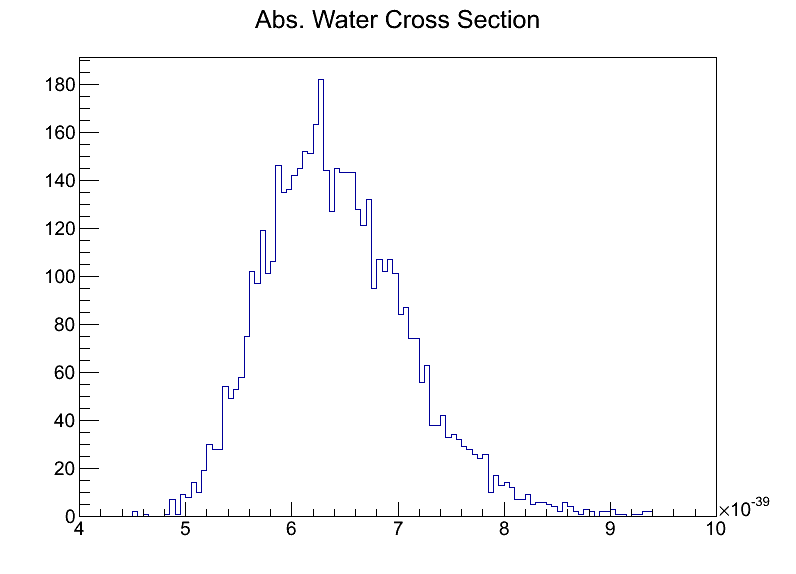
\includegraphics[width=5in]{Figures/fluxvar.png}
\caption{A distribution of the calculated absolute water cross section for 5000 throws of the input flux. The input flux variations are calculated directly from throws of the ND280 bins of the flux covariance matrix.}
\label{fig:fluxvar}
\end{figure}

The cross section error on just the flux term is around $12\%$. However, we measure an overall error of less that $12\%$ on the cross section due to the subtraction method used. There is a larger fraction of out-of-fiducial background in the water-out selection than in the water selection. The background terms increase linearly with total integrated flux, whereas the efficiency terms remain roughly invariant as a function of flux. When calculating total expected signal events in water-in and water-out (N-B/eff.), the final value therefore varies inversely with the integrated flux term variation. However, the total expected signal in water-in data has a smaller variation that the signal in water-out due to smaller background fraction. So in effect, the total expected signal in water-only increases as integrated flux increases and decreases as integrated flux decreases. This correlation yields a smaller error due to flux uncertainty in this subtraction method.

\subsection{Cross Section Model Systematic Uncertainty}
\label{sec:xsecsyst}

The systematic uncertainty from the cross section model is another large contributor of error in this cross section measurement. To evaluate this error, we use reweighting software called T2KReWeight. This software was developed by several T2K working groups working together, and we were not directly involved with its development. This Section covers how we use T2KReWeight to propagate external physics model uncertainties to our absolute cross section measurement. Ideally, for every small variation in a cross section parameter, the MC would be regenerated. Then the particles would be repropagated and the events reconstructed and reselected. However, this is computationally intractable. Instead, the T2KReWeight software calculates the resulting MC variations on the fly by using precalculated response functions. 

For a variation in a physics parameter, the theoretical cross section in NEUT is recalculated. The ratio of the recalculated cross section and the nominal cross section is stored. This procedure is repeated for multiple variations in each physics parameter, storing the cross section ratios for each. This is handled by the reweighting capabilities of the neutrino generator being used, in this case NEUT. Afterwards, T2KReWeight takes a MC neutrino interaction, and based on the interaction type and other truth kinematics, uses the cross section ratios to calculate an event weight that is a ``reweighting" of the nominal event. This weight is directly related to the cross section ratio and is essentially a multiplicative factor describing the change in probability of the event occurring. As the MC truth information is available at all times, event weights can be generated at any given time, without needing to reprocess terabytes of data. Furthermore, while varying parameters like $M_A^{QE}$ requires help from NEUT, most of the cross section parameters are normalization factors. These factors are basically weights already as they can be directly applied to all events from a specific interaction mode (i.e. an increase in the CCQE normalization parameter of $10\%$ means an increase in the CCQE content of our samples by $10\%$ also). This reweighting method is used to quickly evaluate the effect of cross section model uncertainties on our measurement.

 The parametrization of the cross section model and the size of the corresponding errors were discussed in Section \ref{sec:evsim}. There are two types of cross section model uncertainties that were propagated. The first type are uncertainties in the 4-vector generation at the neutrino interaction vertex and the second type are the uncertainties in interactions that occur as a generated particle travels through the nucleus. The latter type of uncertainties are referred to as Final State Interaction (FSI) errors and are evaluated separately.

To estimate the neutrino interaction cross section model uncertainties, for each parameter, we generate an event weight for each selected Monte Carlo CC inclusive event and for each unselected true Monte Carlo CC inclusive event using T2KReWeight. The re-weighted Monte Carlo events will produce a new event cross section evaluated for a 1-sigma parameter excursion divided by the nominal parameter cross section. This is done for each parameter by evaluating weights at a $\pm$1-sigma excursion. Once each selected and unselected event has a weight, we re-evaluate the MC predicted backgrounds and efficiencies and finally the cross-section. The final error for each parameter leads to a fractional shift in the nominal cross section value

\begin{equation}
\delta(\sigma) = \frac{\sigma^{var.}-\sigma^{nom}}{\sigma^{nom}}.
\end{equation}

The positive and negative errors from each parameter variation are shown in Table \ref{tab:XSecPar}. The addition of these errors is not a straightforward task however, especially as the cross section parameters themselves are correlated. Ideally, we would take a throw from the correlation matrix in Figure \ref{fig:xseccorr} for the single pion fit parameters and use gaussian throws for the rest to perform the reweighting procedure multiple times. The resulting distribution of the water cross section values would then yield a total error from physics model uncertainty. This process is unfortunately too computationally intensive, so we use a simpler method. We note that the only two parameters from the single pion fit that affect the measurement appreciably are $M_A{RES}$ and CC 1$\pi$ normalization. The other single pion parameters are either not highly correlated or do not affect the water cross section. Looking closely at the $M_A^{RES}$ parameter, we find that if it increases (decreases), the cross section value decreases (increases). On the other hand, when the CC 1$\pi$ normalization increases (decreases), the cross section value also increases (decreases). Since $M_A^{RES}$ and the CC 1$\pi$ normalization are anti-correlated, upward excursions of $M_A^{RES}$ would suggest downward excursions of CC 1$\pi$ normalization. This is consistent with the cross section decreasing only. Similarly, a downward excursion of $M_A^{RES}$ would suggest an upward excursions of CC 1$\pi$ normalization, yielding an increase in the cross section. So conservatively, we linearly add the fractional cross section change from negative excursions of both parameters. The same is done for the positive excursions. From the values in the last two columns of Table \ref{tab:XSecPar}, this results in a combined $M_A^{RES}$ and CC 1$\pi$ normalization error of $+3.57\%$ and $-3.75\%$.

The rest of the parameters are assumed completely uncorrelated. Even though upward and downward excursions of each parameter cause the cross section to change in different directions, all the remaining errors are added in quadrature. Figures \ref{fig:xsvar1} and \ref{fig:xsvar2} shows the fractional change in the signal efficiency and background rate as a function of the Z vertex position binned by p0dule number. Only water-in MC is shown as the water-out results look very similar. Each plot has the $\pm 1 \sigma$ variation results for a single standard interaction cross section parameter. As the background rate and signal efficiencies are very small in certain regimes, the fractional change varies wildly in those areas, but have little impact on the final cross section measurement. The final systematic uncertainty due to the interaction physics model is $+8.78\%$ and $-13.43\%$. 

\begin{table}[h]
\centering
\caption{Cross section model parameter uncertainties and the resulting absolute water-only cross section fractional error.}
\begin{tabular}{lcccc}\toprule\midrule
\renewcommand{\arraystretch}{1.1}
Parameter &  Value & Error & + Var. (\%) & - Var. (\%)
\\ \midrule
M$_A^{QE}$ & 1.21GeV$^2$ & 0.45 GeV$^2$ & 3.9 & -7.33\\
\midrule
M$_A^{RES}$ & 1.16GeV$^2$ & 0.11 GeV$^2$ & 0.86 & -0.89\\
\midrule
Spectral Function & off & on/off & 0 & -4.01\\
\midrule
Fermi Momentum & 217 MeV/c  & 30 MeV/c & 0.81 & -0.77\\
\midrule
Pionless Delta Decay & 0.2 & 0.2 & 0.21 & -1.05\\
\midrule
DIS/Multi-Pi Shape & 1.0 & 0.4 &  0.46 & -0.44\\
\midrule
CC QE Norm. (E$_\nu < 1.5$~GeV) & 1.0 & $0.11$ & 2.81 & -2.90\\
\midrule
CC QE Norm. (3.5~GeV$>$ E$_\nu > 1.5$~GeV) & 1.0 & $0.30$ & 1.83 & -1.73\\
\midrule
CC QE Norm. (E$_\nu > 3.5$~GeV) & 1.0 & $0.3$ & 1.75 & -1.66\\
\midrule
CC Res Norm. (E$_\nu < 2.5$~GeV) & 1.63 & $0.43$ & 2.71 & -2.85\\
\midrule
CC Res Norm. (E$_\nu > 2.5$~GeV) & 1.0 & $0.4$ & 5.65 & -4.80\\
\midrule
CC Coh Norm. & 1.0 & $1.0$ & 1.42 & -1.31\\
\midrule
%NC COh Norm. & 1.0 & $0.3$ & 0.01 & -0.01\\
%\midrule
%NC 1Pi Norm. & 1.0 & $0.3$ & 0.01 & -0.01\\
%\midrule
NC Other Norm. & 1.0 & $0.3$ & 0.24 & -0.24\\
\midrule
MiniBoone CC 1Pi E$_\nu$ Shape. & off & on/off & 0.0 & -7.45\\
\midrule
\midrule
Total Interaction Systematic & &&$+8.78\% $  & $-13.43\%$  \\
\midrule
\bottomrule
\end{tabular}
\label{tab:XSecPar}
\end{table}

\newpage
\clearpage
\begin{figure}[h]
\centering
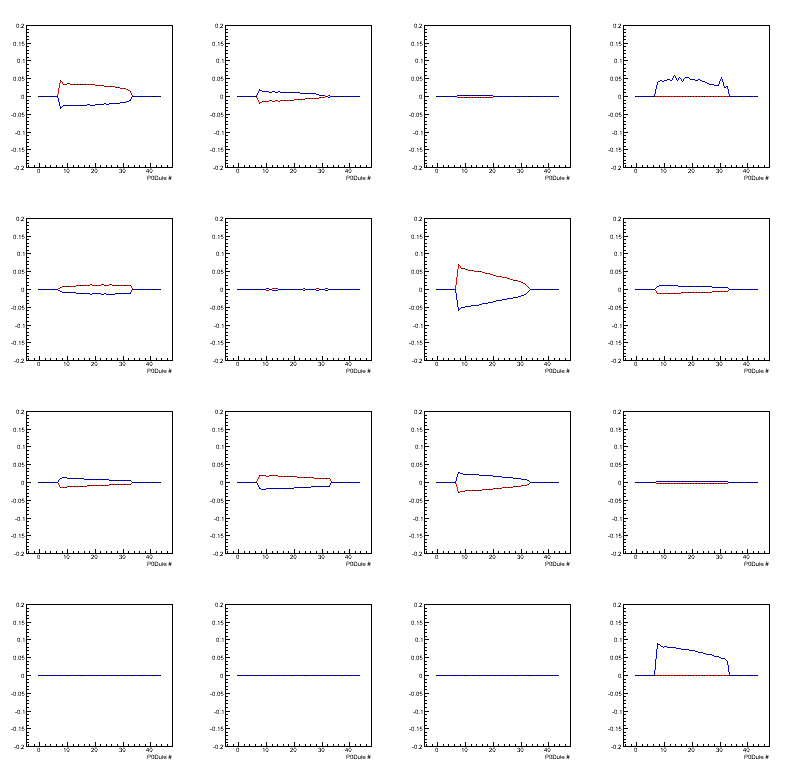
\includegraphics[width=5in]{Figures/TN100Plots/c_6_0.png}
\caption{The fractional change in the water-in signal efficiency (predicted from MC) as a function of p0dule number of neutrino interaction vertex for a +1 $\sigma$ (blue) and -1$\sigma$ (red) variation of cross section parameter. From left to right, top to bottom, the cross section parameters varied are: MAQE, MARES, DIS Multi-Pi Shape, Spectral Function, Fermi Momentum, Pion-less Delta Decay, CCQE Norm. ($E_\nu < 1.5$GeV), CCQE Norm. ( 3.5~GeV$E_\nu>1.5$GeV), CCQE Norm ($E_\nu > 3.5$GeV), CC 1Pi Norm. ($E_\nu < 2.5$GeV), CC 1Pi Norm. ($E_\nu > 2.5$GeV), CC Coh Norm., NC Coh Norm., NC 1Pi Norm., NC Other Norm., MiniBoone CC 1Pi $E_\nu$ Shape.}
\label{fig:xsvar1}
\end{figure}

\newpage
\begin{figure}[h]
\centering
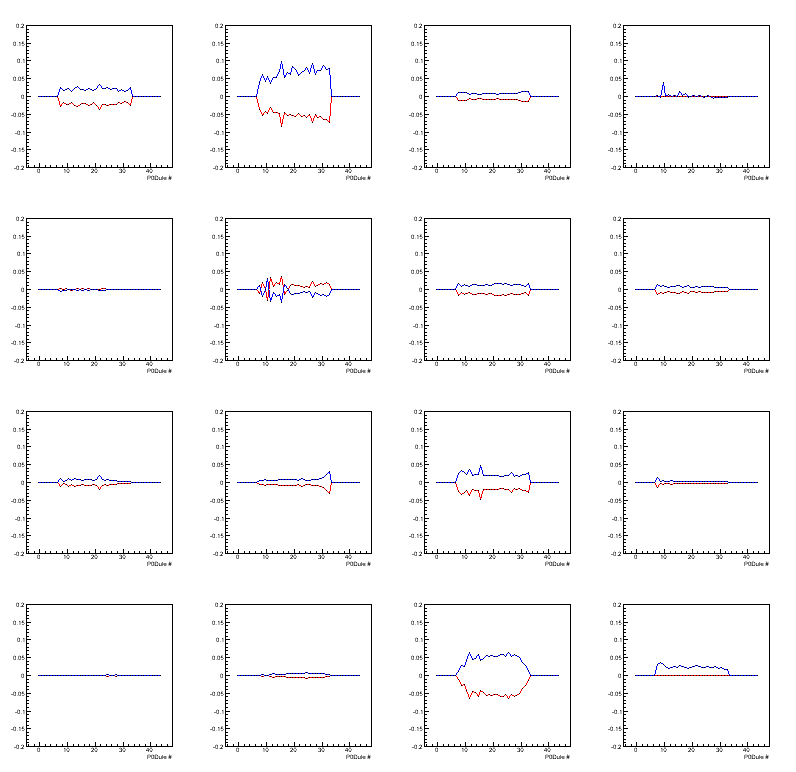
\includegraphics[width=5in]{Figures/TN100Plots/c_12_0.png}
\caption{The fractional change in the water-in background (predicted from MC) as a function of p0dule number of neutrino interaction vertex for a +1$\sigma$ (blue) and -1$\sigma$ (red) variation of cross section parameter. From left to right, top to bottom, the cross section parameters varied are: MAQE, MARES, DIS Multi-Pi Shape, Spectral Function, Fermi Momentum, Pion-less Delta Decay, CCQE Norm. ($E_\nu < 1.5$GeV), CCQE Norm. ( 3.5~GeV$E_\nu>1.5$GeV), CCQE Norm ($E_\nu > 3.5$GeV), CC 1Pi Norm. ($E_\nu < 2.5$GeV), CC 1Pi Norm. ($E_\nu > 2.5$GeV), CC Coh Norm., NC Coh Norm., NC 1Pi Norm., NC Other Norm., MiniBoone CC 1Pi $E_\nu$ Shape.}
\label{fig:xsvar2}
\end{figure}

The FSI error is evaluated following the procedure in Section \ref{sec:evsim}. There are 16 combinations of variations used for the FSI parameters to fully account for the necessary uncertainty. Each combination of 16 parameter variations is fed through T2KReWeight and the water cross section is recalculated. The fractional change from the nominal cross section is given as the error as before. The water cross section error from each combination are averaged together to yield the FSI uncertainty contribution. The results are shown in Table \ref{tab:XSecFSI}.

\begin{equation}
\sigma_{avg}^2 = \sum_i^{16} \frac{\sigma_i^2}{16}
\end{equation}

\begin{table}[h]
\caption{Final State Interaction parameter uncertainties and the resulting water-only cross section fractional error.}
\centering
\begin{tabular}{cccccccc}\toprule\midrule
\renewcommand{\arraystretch}{1.1}
Comb.& Inel Lo & Inel Hi & Pi Prod. & Pi Abs. & Ch Ex Lo & Ch Ex Hi & Error
\\ \midrule
1 & 0.6 & 1.1 & 1.5 & 0.7 & 0.5 & 2.3 & 0.23\%\\
\midrule
2 & 0.6 & 1.1 & 1.5 & 0.7 & 1.6 & 2.3 & 0.56\%\\
\midrule
3 & 0.7 & 1.1 & 1.5 & 1.6 & 0.4 & 2.3 & 0.16\%\\
\midrule
4 & 0.7 & 1.1 & 1.5 & 1.6 & 1.6 & 2.3 & 0.27\%\\
\midrule
5 & 1.4 & 1.1 & 1.5 & 0.6 & 0.6 & 2.3 & 0.45\%\\
\midrule
6 & 1.3 & 1.1 & 1.5 & 0.7 & 1.6 & 2.3 & 0.33\%\\
\midrule
7 & 1.5 & 1.1 & 1.5 & 1.5 & 0.4 & 2.3 & -0.44\%\\
\midrule
8 & 1.6 & 1.1 & 1.5 & 1.6 & 1.6 & 2.3 & -0.03\%\\
\midrule
9 & 0.6 & 2.3 & 0.5 & 0.7 & 0.5 & 1.3 & 0.46\%\\
\midrule
10 & 0.6 & 2.3 & 0.5 & 0.7 & 1.6 & 1.3 & 0.34\%\\
\midrule
11 & 0.7 & 2.3 & 0.5 & 1.6 & 0.4 & 1.3 & 0.30\%\\
\midrule
12 & 0.7 & 2.3 & 0.5 & 1.6 & 1.6 & 1.3 & 0.30\%\\
\midrule
13 & 1.4 & 2.3 & 0.5 & 0.6 & 0.6 & 1.3 & 0.30\%\\
\midrule
14 & 1.3 & 2.3 & 0.5 & 0.7 & 1.6 & 1.3 & -0.01\%\\
\midrule
15 & 1.5 & 2.3 & 0.5 & 1.5 & 0.4 & 1.3 & -0.37\%\\
\midrule
16 & 1.6 & 2.3 & 0.5 & 1.6 & 1.6 & 1.3 & -0.31\%\\
\midrule
Total & & & & & & & 0.34\%\\
\midrule
\bottomrule
\end{tabular}
\label{tab:XSecFSI}
\end{table}

The total error in the absolute water cross section measurement is +8.79\% and -13.43\% when FSI and standard interaction uncertainties are added in quadrature. We note that there is some model dependence in our measurement that is introduced through the MC estimate of the background interactions. Also, a majority of the background contamination is OOFV CC inclusive events. As this background still consists of CC inclusive events (albeit outside the fiducial volume) we are using the MC to model not only the contamination rate of the OOFV events, but also the rate of CC inclusive events. This implies that there is some signal model dependence in our measurement. As the variation of $M_A^{QE}$, a parameter that controls a signal interaction mode, caused a 7\% shift in the cross section measurement, the model dependence is not negligible.

\newpage